\PassOptionsToPackage{hyphens}{url}
\documentclass[a4paper,fleqn]{cas-dc}
\usepackage[authoryear,longnamesfirst]{natbib}
\usepackage{amsmath,amssymb,booktabs,array}
\usepackage{graphicx}
\usepackage{url}

% Two narrow columns leave TeX little room; a small stretch avoids
% overfull boxes of a few points without visibly loosening the type.
\emergencystretch=1em

% cas-common sets the keywords box into a zero-width hbox without \hss, which TeX reports as a
% 123.6 pt overfull box at \maketitle. Same environment with \hss added: identical output.
\ExplSyntaxOn
\RenewDocumentEnvironment { Abstract } { o }
{
  \group_begin:
  \IfNoValueTF { #1 } { }
  { \tex_gdef:D \abstractname { #1 } }
  \parindent \c_zero_dim
  \box_if_empty:NTF \g_stm_key_box
  { \leftskip = .35 \textwidth }
  {
    \dim_gset:Nn \l_tmpa_dim { \box_ht:N \g_stm_key_box }
    \dim_gadd:Nn \l_tmpa_dim { \box_dp:N \g_stm_key_box }
    \leftskip .35\textwidth
    \hspace*{-.35 \textwidth }
    \noindent\hbox_to_wd:nn { \c_zero_dim } { \box \g_stm_key_box \hss }
    \skip_vertical:n { - \l_tmpa_dim }
  }
  \noindent \abstractname \par
  \skip_vertical:n { -4pt}
  \noindent \rule{.65\textwidth}{.2pt}\par \footnotesize
  \ignorespaces \everypar { \parindent=1.5em }
}
{ \par \group_end: }

% cas-common hard-codes "Preprint submitted to Elsevier" in the footer. This is an SSRN working
% paper, not an Elsevier submission, so the footer names the version instead.
\cs_set:Npn \__first_footerline:
{
  \group_begin:
  \small
  \sffamily
  \ifnum\theblind>0\relax
  \else
    \__short_authors: :~
  \fi
  { \rmfamily \itshape Working~paper,~\today }
  \group_end:
}
\ExplSyntaxOff

% Placeholder for a number or a sentence that the registered analysis has not produced yet.
% Every \PH{key} is listed with the file it will be filled from in docs/paper2/MANUSKRIPT.md.
% Rule: every number in this file comes from results/p2 or from the pre-registration, or it is a \PH.
\newcommand{\PH}[1]{\textbf{[#1]}}

\begin{document}

\shorttitle{What does the edge cost?}
\shortauthors{G. Albiez}

\title[mode=title]{What does the edge cost? Capital-adjusted market making under a public portfolio-margin engine}

\author[1]{Gregor Albiez}[orcid=0009-0006-6036-4932]
\ead{gregor.albiez@students.fhnw.ch}
\affiliation[1]{organization={University of Applied Sciences and Arts Northwestern Switzerland (FHNW)},
                country={Switzerland}}

\begin{abstract}
A market maker quotes against a budget of capital, not of contracts, yet its edge is almost always reported
per contract. On Derive the rule that turns a book into required capital is public: a deterministic margin
engine with parameters stored on chain. I measure capital by evaluating that engine on hypothetical
portfolios, not on account balances: a single contract for each of \PH{n-fills} option fills studied in a
companion paper, and the actual books of the ten dominant maker subaccounts, under each of the venue's three
margin managers. Per unit of portfolio-margin capital, the net edge ranks the cells of the
moneyness-by-tenor map with a rank correlation of \PH{h1-rho} to its ranking per unit of notional. Inside a
dominant maker's book the next contract binds a median \PH{h2-median} of its stand-alone capital, and
standard margin needs \PH{h3-median} times the capital of portfolio margin for the same books. When a
parameter change made capital cheaper, the half spread \PH{h4-direction}. Four hypotheses were registered
before any capital figure was computed; \PH{n-rejected} are rejected.
\end{abstract}

\begin{keywords}
market microstructure \sep options \sep portfolio margin \sep market making \sep funding constraints
\sep decentralised exchange \sep pre-registration \sep JEL: G13, G12, G24, D47
\end{keywords}

\maketitle

\section{Introduction}\label{sec:intro}
A market maker on an options venue does not run out of contracts. It runs out of capital. The deposit
behind the margin on its positions is the input on which funding constraints act \citep{brunnermeier2009}
and which margin-based pricing turns into a required return \citep{garleanu2011}. The literature on market
making nonetheless counts in contracts. Inventory models bound the position in units
\citep{ho1981,avellaneda2008,gueant2013}, option market making prices the risk of the book
\citep{stoikov2009,garleanu2009}, the option spread compensates for risks the maker cannot hedge
\citep{jameson1992}, and inventory risk moves option prices \citep{muravyev2016}. Even the illiquidity
premium in options is measured against the price of the option \citep{christoffersen2018}. What a unit of
edge costs in capital is left open, because on most venues the capital a book requires is visible only to
the account that holds it.

Derive makes it observable. The venue margins every subaccount under one of three managers: a strategy-based
standard manager (SM), a legacy portfolio manager and a second-generation portfolio manager (PM2). Each is a
deterministic function of the positions, the venue's price feeds and risk parameters stored on chain, and a
public endpoint evaluates it for any hypothetical book without an account. Capital can therefore be computed
for books nobody held, at past blocks, and under a manager the book was never in. I use that property to
measure capital on hypothetical portfolios evaluated by the venue's own engine, not on account balances that
mix what a book needs with whatever a trader chooses to deposit.

The question is the one \citet{albiez2026} leaves open. That paper maps the maker's net edge over moneyness
and tenor, per contract and per unit of notional. Here the same fills are priced in capital: how much
capital does the edge bind, and does the map change when the edge is measured per unit of capital? Option
strategies are known to lose much of their appeal to investors once margin is charged
\citep{santaclara2009}. This paper takes the maker's side and uses the rule the venue actually applies.

Four contributions follow. The first is a capital map: the edge per unit of capital over the
moneyness-by-tenor grid of \citet{albiez2026}, computed with the engine itself rather than with a margin
model of my own. The second is the marginal cost of a fill, the capital a fill adds to the actual book of a
dominant maker under the manager that account used. The third is the value of netting: the capital of the
same real books under standard margin, legacy portfolio margin and PM2, in the tradition that compares
strategy-based and portfolio margining on identical positions \citep{kupiec1996}. The fourth is a price of
capital. That the balance sheets of market makers move liquidity is known from their inventories and
revenues \citep{comertonforde2010}. Here, parameter changes are on-chain events whose effect on the capital
of every cell can be computed exactly, which turns them into a natural experiment with a known dose.

Four hypotheses were registered before the first capital figure was computed. H1 holds that the capital
denominator reorders the map, so that edge per notional and edge per unit of PM2 capital rank the cells
differently. H2 holds that inside a dominant maker's book the next contract is cheap, binding less than half
of its stand-alone capital. H3 holds that PM2 saves more than half of the capital that standard margin
requires for the same books. H4 holds that when a parameter change makes capital cheaper, the half spread
falls.

% intro-results: one sentence per hypothesis with verdict and headline number, written once the registered
% tests have run. Keep the order H1 to H4.
\PH{intro-results}

\section{The engine and what it returns}\label{sec:engine}
The standard manager is strategy based. Each option is margined in isolation, each expiry takes the smaller
of that sum and its maximum loss, and expiries are added up. A long option earns no credit of its own, so
under SM the capital of a long book is its full premium. The legacy manager and PM2 are scenario engines in the
spirit of SPAN \citep{kupiec1994}: the book is revalued under spot and volatility shocks, and the worst loss
plus contingencies is the requirement. PM2 adds skew shocks, a static discount on position values and a
rate feed. Both net within one underlying and never across, and the scope of netting decides what it saves
\citep{duffie2011,cont2014}. Scenario margin goes back to \citet{figlewski1984}, and its worst-loss form is
a coherent risk measure \citep{artzner1999}. Unusually, the rule is public code with public parameters,
as in the lending protocols of \citet{qin2021}, not the private schedule of a centralised venue
\citep{soska2021}.

The public endpoint \texttt{get\_margin} does not return a requirement. For positions $q$ and USDC
collateral $C$ it returns, for initial and for maintenance margin $X$,
\begin{equation}
  \mathrm{net}_X(q;C) = C + V(q) - R_X(q),
\end{equation}
with $V$ the value of the positions in the manager's own valuation and $R_X$ the requirement; a book is
admissible when its initial net margin is not negative. The field \texttt{pre} evaluates the book as given
and \texttt{post} the book after simulated changes, both at one price state within one request. That is
what makes a marginal cost measurable: two requests would also compare two prices.

The quantity used throughout is the capital needed to open a book $q$ at traded prices $p$ and meet initial
margin,
\begin{equation}
  K_p(q) = \sum_{i \in \text{options}} p_i\,q_i - \mathrm{net}_{\mathrm{IM}}(q;0).
\end{equation}
Collateral enters net margin one for one, so $K_p$ is the deposit at which the book is exactly admissible
once the premium has changed hands. It needs no valuation of its own, and $K_p - R_{\mathrm{IM}} = \sum p_i q_i - V$
is a valuation convention, not capital. Perpetuals carry no premium. For a trade $\Delta q$ at prices $p$,
one request with a collateral change of $-p\,\Delta q$ gives $\Delta K = -(\mathrm{post} - \mathrm{pre})$.
Figure~\ref{fig:t1} shows $K_p$ for single contracts on the BTC surface.

\begin{figure*}[t]
  \centering
  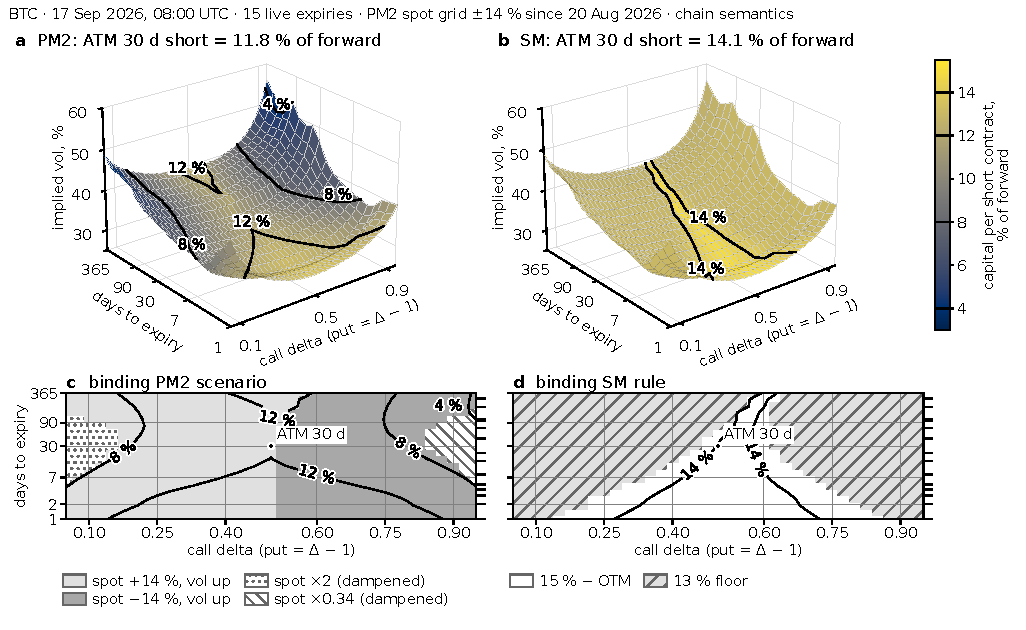
\includegraphics[width=\linewidth]{figures/t1.pdf}
  \caption{\textbf{The surface as the engine sees it.} BTC implied volatility over moneyness and tenor at
  block \PH{t1-block}, as written on chain. The colour is the capital in USDC that one short contract binds
  under PM2 (panel a) and under standard margin (panel b), on a common scale, so height and colour come from
  the same block.}
  \label{fig:t1}
\end{figure*}

Two engines implement the managers. The off-chain engine behind the endpoint is the one
the venue trades on. Its PM2 discounts at a flat rate the documentation does not mention, which a box spread
in each of the fourteen listed BTC expiries on 24 September 2026 puts at two per cent to within
$2.7\times10^{-7}$. The on-chain engine settles and liquidates, and discounts with the rate feed, which ranged
from 3.64 to 3.82 per cent across the same expiries. Only the on-chain semantics can be reconstructed for
past blocks, so the history here uses parameters and feeds as they stood at the block, and the off-chain
rate serves only as a present-day sensitivity.

Reading $C - \mathrm{net}$ as the requirement is tempting and wrong: it equals $R - V$ and mixes the value
of the positions into the margin. It produced contradictory numbers in the probes that preceded this paper.
A near-the-money book, alternating long and short across the term structure, gave a ratio of standard to
PM2 margin of 11.86 on $C - \mathrm{net}$ at block 44\,810\,149 on 17 September 2026. A book of the
shortest expiries with random signs and deep in-the-money wings gave 1.19 at block 45\,110\,142 a week
later. On $R$ at the same blocks the ratios are 10.76 and 2.14 (Figure~\ref{fig:t2}). Every parameter
getter returns identical values at both blocks, so the remaining gap is the book, not the engine. The rest
was $V$: the second book had a PM2 value of $-496\,859$ USDC, which adds the same amount to both numerators
and pulls the ratio towards one. Netting factors are properties of books, which is why this paper measures
them on real ones.

\begin{figure*}[t]
  \centering
  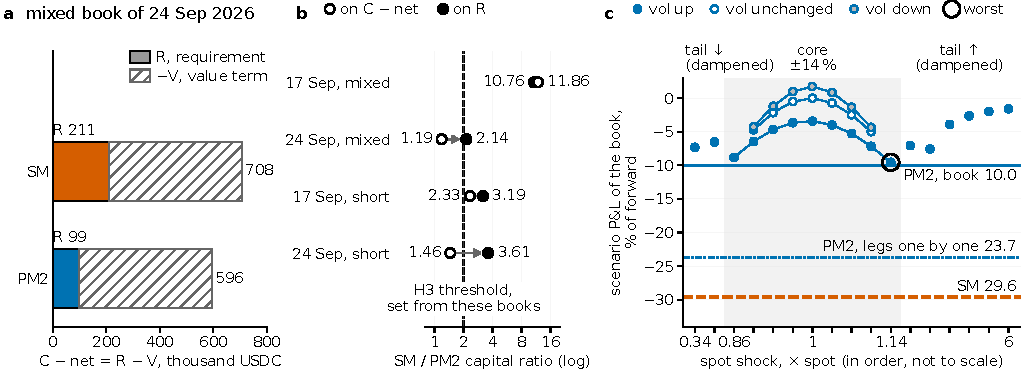
\includegraphics[width=\linewidth]{figures/t2.pdf}
  \caption{\textbf{What \texttt{get\_margin} returns.} Panel a splits net margin into collateral, value and
  requirement, $\mathrm{net} = C + V - R$, for one book. Panel b sets the ratio of standard to PM2 margin
  read as $C - \mathrm{net}$ against the ratio on $R$ for the probe books of 17 and 24 September 2026 at
  their historical blocks: 11.86 against 10.76 and 1.19 against 2.14 for the mixed books, 2.33 against 3.19
  and 1.46 against 3.61 for books that are short throughout. The two bars of one book differ only
  through the value $V$, which enters $C - \mathrm{net}$ and not $R$.}
  \label{fig:t2}
\end{figure*}

\section{Data and measurement}\label{sec:data}
The fills are those of \citet{albiez2026}: every BTC, ETH and HYPE option fill from 11 January 2024 to
\PH{sample-end}, \PH{n-fills} in all, each with the maker's side, price, size and the net edge thirty
minutes after the fill in USDC per contract. SM covers the whole sample, for HYPE from 11 November 2025; the legacy manager covers BTC and ETH
throughout; PM2 covers BTC and ETH from 12 June 2025 23:00 UTC and HYPE from 11 November 2025. That span
is the PM2 window of an underlying, and every test runs inside it.

The market state of a fill is rebuilt from the venue's feed events at its block: spot and, per expiry, the
forward, the SVI curve and the PM2 rate, each at the last value pushed before the block. No fill is dropped for a stale feed; the age is
carried along. Parameters are read with the managers' getters at every block where an update event fired.
The legacy manager emits no events, so its changes are located by bisection. Figure~\ref{fig:f5} shows the
resulting timelines.

Capital per fill is that of a book holding only the fill: $q = +1$ when the maker bought and $q = -1$ when
it sold, at the fill price, under every manager available at the block. Initial margin is primary and
maintenance margin a sensitivity. A cell is an
underlying, a maker side, an absolute delta bucket and a tenor bucket from \citet{albiez2026}, occupied from
200 fills. Its edge per unit of capital and per unit of notional are ratios of sums in basis points,
\begin{equation}
  e^{K}_c = 10^4\,\frac{\sum_{i \in c} NE_i\,a_i}{\sum_{i \in c} K_i\,a_i}, \qquad
  e^{N}_c = 10^4\,\frac{\sum_{i \in c} NE_i\,a_i}{\sum_{i \in c} S_i\,a_i},
\end{equation}
with $NE$ the net edge, $a$ the size and $S$ the index price.

The maker books are those of the ten subaccounts with the most maker fills. Their holdings and manager are
read on chain at the first block of each UTC day; the book before a fill adds every earlier fill of the
subaccount on that day and drops expired options. The marginal cost of a fill is
$\Delta K = K(\text{after}) - K(\text{before})$ under the account's manager and library, with existing
positions at the on-chain mark and the new contract at its fill price, relative to the stand-alone capital
of the same contract. The netting value of a maker-day is the capital of its opening book under SM over
that under PM2, each underlying computed separately and summed. Subaccounts appear in every result only as
hashes.

For H4 each parameter change becomes a dose: $d_{c,e}$ is the mean of $\log(K_{\text{after}} /
K_{\text{before}})$ over the fills of cell $c$ in the fourteen days before event $e$, both capitals pricing
the same fill in the same market state with the parameters after and before the event. Events whose largest
absolute dose is below one per cent are dropped. The outcome is the half spread in basis points of the
index, and over fourteen days on either side of the event, without the event day,
$y_i = \alpha_{c,e} + \gamma_{t,u} + \beta\,\mathrm{post}_i\,d_{c,e} + \varepsilon_i$.

Intervals are percentile intervals of a cluster bootstrap over UTC days with 9\,999 draws; for H1 each draw
recomputes both cell measures and the correlation. H4 uses a wild cluster bootstrap with Rademacher weights
and restricted residuals, and 100 placebo dates at least 28 days from any event. Before any capital entered
a test, the offline replicas were checked against \texttt{eth\_call} on the deployed contracts, on at least
48 random blocks per underlying and manager and on 20 maker-days, against registered thresholds of 0.1 per
cent for the median absolute relative deviation of $K$ and 1 per cent for its 95th percentile. The median is
\PH{val-median} and the 95th percentile \PH{val-p95} (Figure~\ref{fig:a1}).

\section{Results}\label{sec:results}

\subsection{The capital denominator and the map (H1)}
Figure~\ref{fig:f1} shows what a single contract costs under each manager across absolute delta and tenor.
% f1-pattern: where the three managers differ most, maker buys against maker sells (from capital_cells.csv).
\PH{f1-pattern}
For a single short contract the ratio of SM to PM2 capital runs from \PH{f1-ratio-min} to
\PH{f1-ratio-max} across occupied cells.

\begin{figure*}[t]
  \centering
  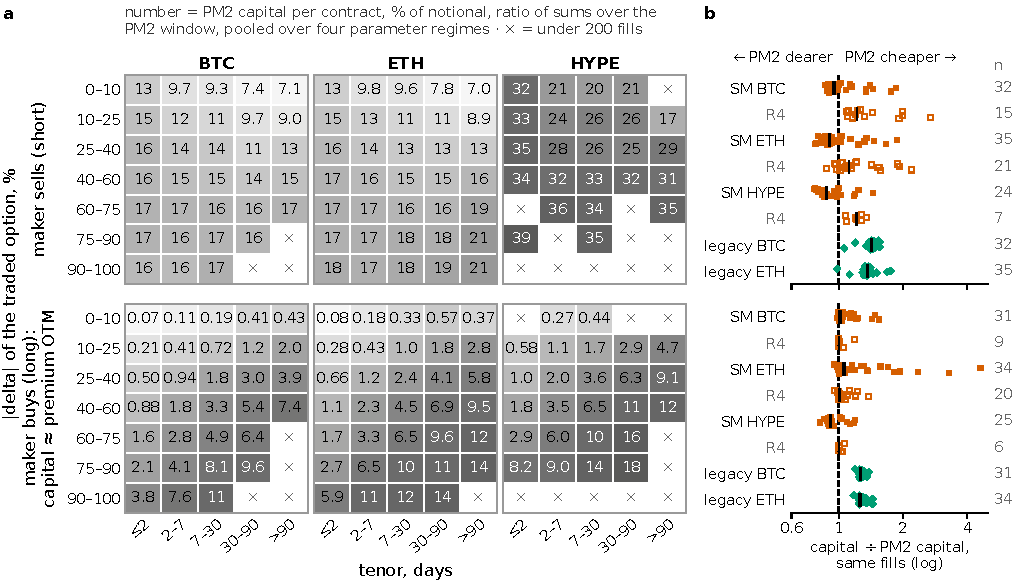
\includegraphics[width=\linewidth]{figures/f1.pdf}
  \caption{\textbf{What one contract costs.} Capital per contract in USDC under standard margin, legacy
  portfolio margin and PM2 over absolute delta and tenor, for maker buys (upper row) and maker sells (lower
  row). Each panel is shaded on its own scale; an empty cross marks a cell with fewer than 200 fills.}
  \label{fig:f1}
\end{figure*}

Figure~\ref{fig:f2} sets the two maps side by side. Across the \PH{h1-cells} occupied cells of the PM2
window, the rank correlation between edge per notional and edge per unit of PM2 capital is
\PH{h1-rho}, with a 90 per cent interval from \PH{h1-lo} to \PH{h1-hi}. The registered rule rejects H1 when
the upper bound reaches 0.5, and H1 is \PH{h1-verdict}.
% h1-reading: which cells change rank most, and whether the reordering runs along tenor, delta or side.
\PH{h1-reading}
Pooled over cells, the edge per unit of PM2 capital is \PH{h1-pooled-sell} basis points for maker sells and
\PH{h1-pooled-buy} for maker buys.

\begin{figure*}[t]
  \centering
  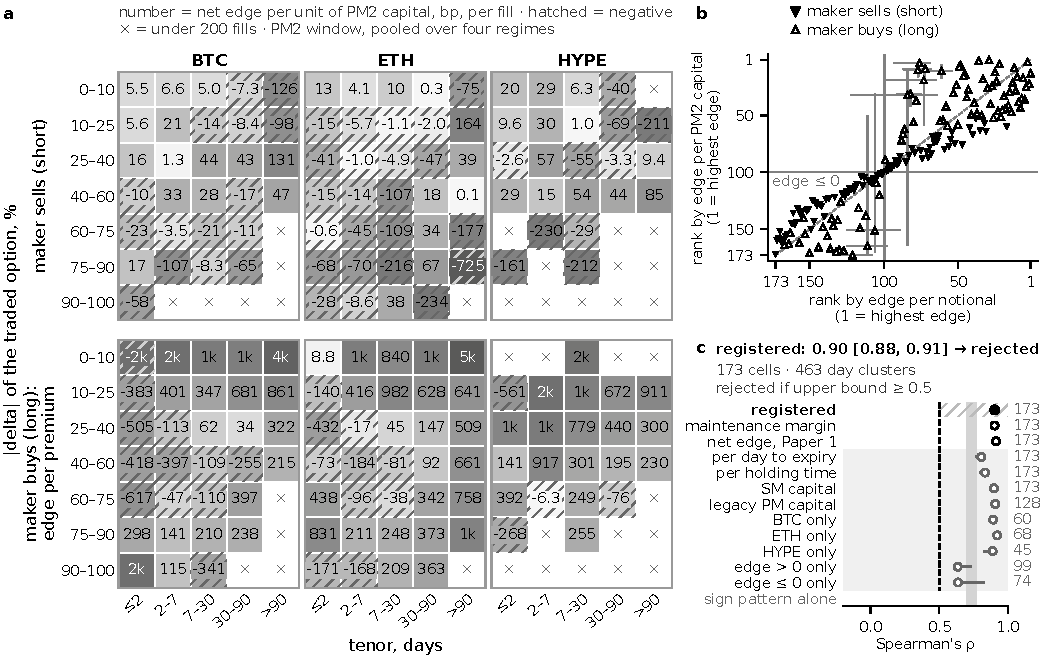
\includegraphics[width=\linewidth]{figures/f2.pdf}
  \caption{\textbf{The map in two denominators.} Edge per notional (left) and edge per unit of PM2 capital
  (right) in basis points, per underlying and maker side in the PM2 window. Lines connect the rank of each
  cell in the two maps, which is the quantity H1 tests; the inset gives $\rho$ with its 90 per cent
  interval.}
  \label{fig:f2}
\end{figure*}

\subsection{The next contract in a maker's book (H2)}
Of the fills of the ten dominant subaccounts in the PM2 window whose account was under PM2 at the start of
the day, \PH{h2-n} enter the test; \PH{h2-excl} have a stand-alone capital that is not positive and are
excluded and counted, as registered.
% h2-sample: one sentence on whether the registered random sample of the fills applied.
\PH{h2-sample}
Figure~\ref{fig:f3} shows the distribution of $\Delta K / K_{\text{single}}$. Its median is
\PH{h2-median}, with a 90 per cent interval from \PH{h2-lo} to \PH{h2-hi}, and \PH{h2-share-nonpos} of the
fills leave the capital of the book unchanged or reduce it. H2 is \PH{h2-verdict}.
% h2-reading: which fills are cheap at the margin (against the book) and which are expensive (with it).
\PH{h2-reading}

\begin{figure}[t]
  \centering
  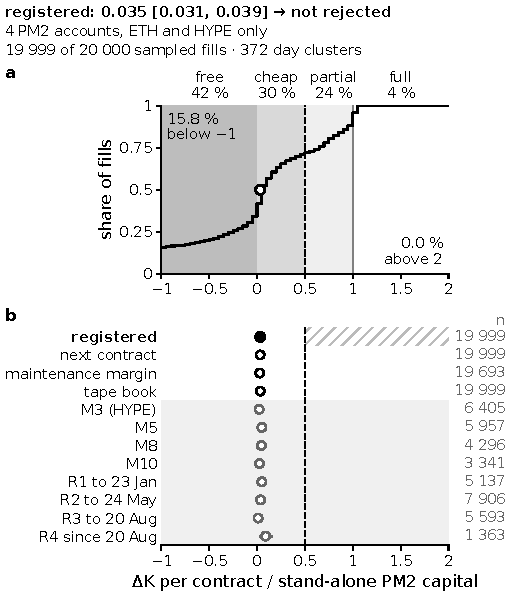
\includegraphics[width=\linewidth]{figures/f3.pdf}
  \caption{\textbf{The next contract in a dominant maker's book.} Distribution of
  $\Delta K / K_{\text{single}}$ under PM2 over the tested fills, with the registered threshold of one half
  and the median with its 90 per cent interval. Mass at or below zero is the share of fills that free
  capital.}
  \label{fig:f3}
\end{figure}

\subsection{What netting is worth (H3)}
Figure~\ref{fig:f4} reports the capital of the same opening books under SM and under PM2 over
\PH{h3-days} maker-days of the PM2 window with at least one option position; \PH{h3-excl} maker-days with a
PM2 capital that is not positive are excluded and counted. The median of $K_{\mathrm{SM}}/K_{\mathrm{PM2}}$ is
\PH{h3-median}, with a 90 per cent interval from \PH{h3-lo} to \PH{h3-hi}. The registered threshold of two
sits at the lower end of the probe books of Section~\ref{sec:engine}, whose ratios on $R$ ran from 2.14 to
10.76 at their historical blocks, and H3 is \PH{h3-verdict}. The legacy manager, shown alongside as an
exploratory comparison, needs \PH{h3-legacy-ratio} times the PM2 capital for the same books.
% h3-reading: dispersion across makers and over time; which books net least.
\PH{h3-reading}

\begin{figure}[t]
  \centering
  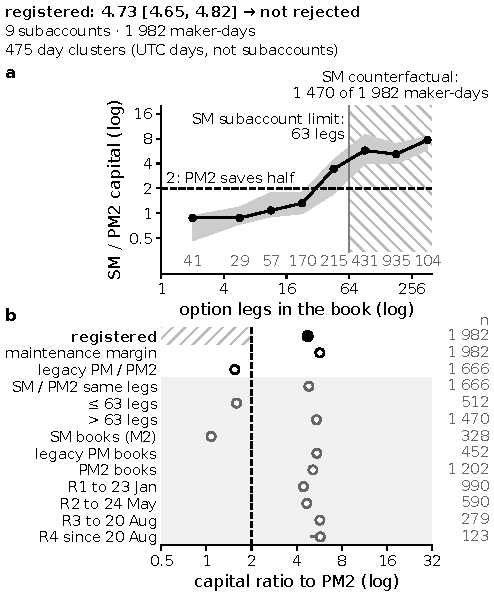
\includegraphics[width=\linewidth]{figures/f4.pdf}
  \caption{\textbf{What netting is worth.} $K_{\mathrm{SM}}/K_{\mathrm{PM2}}$ over maker-days in the PM2 window on a
  logarithmic axis, with the legacy manager alongside. The dashed line is the registered threshold of two.}
  \label{fig:f4}
\end{figure}

\subsection{The price of capital (H4)}
Figure~\ref{fig:f5} places the parameter changes on the calendar next to the managers' shares of open
interest and the capital of a fixed reference book. Of \PH{h4-events-raw} parameter changes in the
registered set, \PH{h4-events} survive the merge and the dose filter, with \PH{h4-cells} cell-event pairs
that have at least 20 fills on each side.
% h4-doses: range and sign of the doses, tightening against loosening.
\PH{h4-doses}
The estimate of $\beta$ is \PH{h4-beta} basis points of the index per unit of log capital, with a one-sided
wild cluster bootstrap $p$ of \PH{h4-p}, and it lies at the \PH{h4-placebo-pct} percentile of the 100
placebo estimates (Figure~\ref{fig:f6}). H4 is rejected unless the estimate is positive at five per cent
and above the 95th placebo percentile; it is \PH{h4-verdict}.
% h4-reading: what the estimate means in basis points of half spread per ten per cent of capital.
\PH{h4-reading}

\begin{figure*}[t]
  \centering
  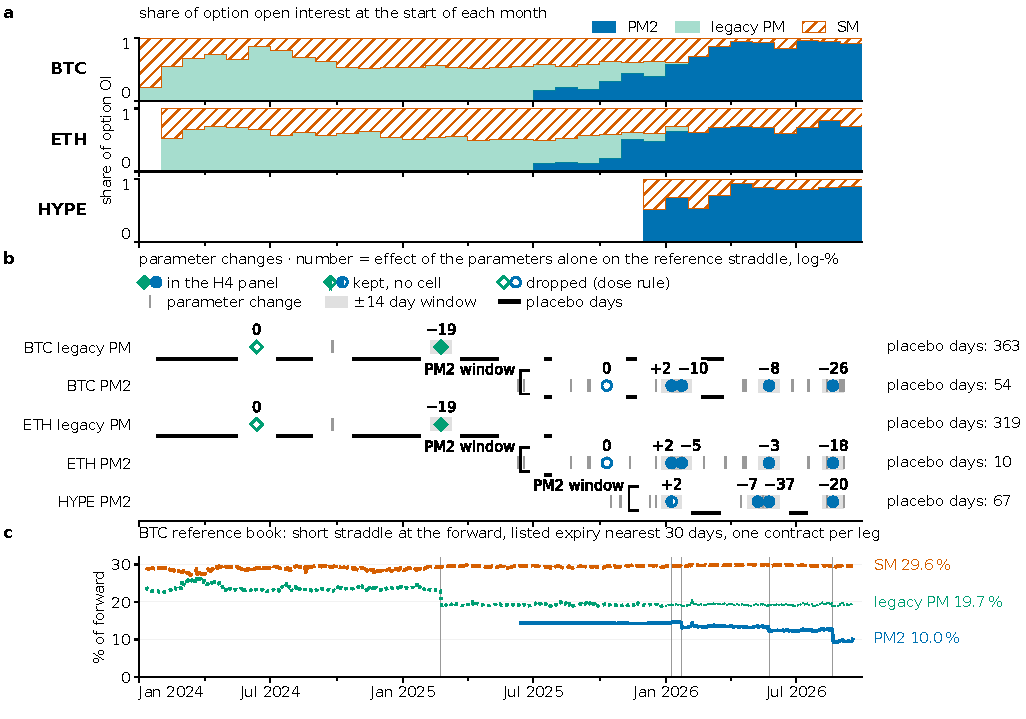
\includegraphics[width=\linewidth]{figures/f5.pdf}
  \caption{\textbf{The engine over time.} Panel a is the share of option open interest per manager. Panel b
  marks the parameter changes per underlying and manager, with the events that enter H4 filled. Panel c is
  the capital of a fixed reference book under each manager, recomputed at every parameter change.}
  \label{fig:f5}
\end{figure*}

\begin{figure*}[t]
  \centering
  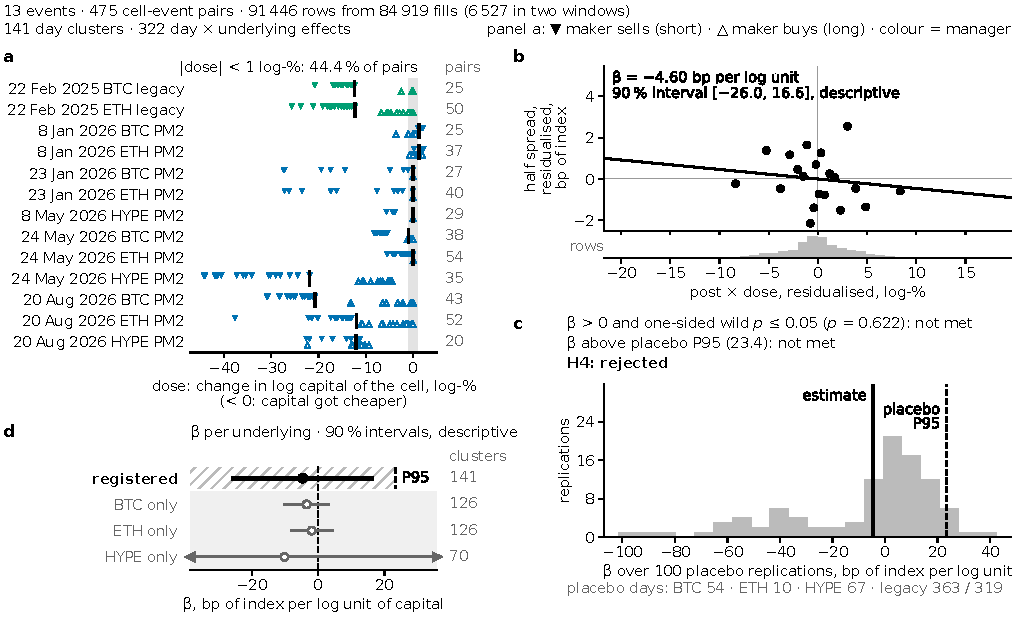
\includegraphics[width=\linewidth]{figures/f6.pdf}
  \caption{\textbf{The price of capital.} Panel a is the change in the half spread against the dose per cell
  and event, binned, with the fitted slope $\beta$. Panel b is the distribution of $\beta$ over the 100
  placebo dates with the estimate marked.}
  \label{fig:f6}
\end{figure*}

\section{Discussion}\label{sec:discussion}
% disc-map: what the capital map changes against the per-notional map of the companion paper (H1).
\PH{disc-map}

% disc-book: what the marginal cost and the netting value imply for how a maker should size and where it
% should run its book (H2, H3).
\PH{disc-book}

% disc-price: whether capital is a price the half spread responds to (H4), read against the inventory and
% funding literature.
\PH{disc-price}

Several limits bound these readings. Capital is measured on hypothetical portfolios, so it is the capital
the engine would require and not what makers deposited; nothing here observes balances. Margin for open
orders, which the venue charges but the endpoint does not return, lies outside the measure, and so does
every external bound on a book: caps on open interest, account limits and depth. The history is in chain
semantics, while the venue trades on the off-chain engine, whose flat discount cannot be reconstructed for
the past; the two differ by a valuation convention that grows with tenor. Collateral other than USDC, which
PM2 credits against positions, is left outside $K$. Edge is a flow and capital a stock, so edge per unit of
capital per fill describes a position held for the life of the fill; normalised by time to expiry or by the
empirical holding period, the map \PH{disc-time}. Finally, some accounts now run under libraries of their
own, which the maker books respect and the single-contract map does not.

\begin{figure*}[t]
  \centering
  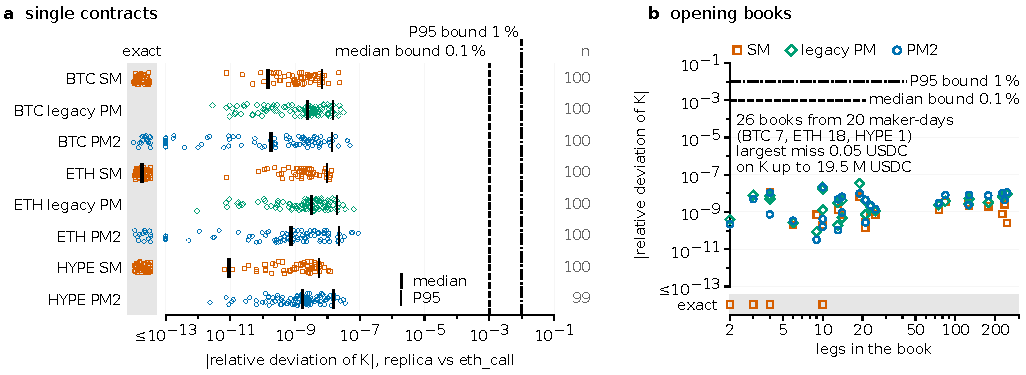
\includegraphics[width=\linewidth]{figures/a1.pdf}
  \caption{\textbf{Does the replica match the chain?} Relative deviation of $K$ between each offline replica
  and \texttt{eth\_call} on the deployed contracts, per underlying and manager, for single contracts (panel
  a) and for maker books (panel b). The dashed lines are the registered thresholds of 0.1 and 1 per cent.}
  \label{fig:a1}
\end{figure*}

\section{Conclusion}\label{sec:conclusion}
On Derive the capital behind a quote is not a private number. The engine that sets it is public code with
parameters on chain, so the capital of any book can be computed at any block, including books nobody held.
% concl-results: one sentence per hypothesis in plain words, with the headline number.
\PH{concl-results}
Four hypotheses were registered before any capital figure existed, and \PH{n-rejected} are rejected.
% concl-close: the one sentence a maker should take away.
\PH{concl-close}

\section*{Data, code and pre-registration}
Every input to this paper is public. The fills come from the venue's public trade tape as in
\citet{albiez2026}; feeds, parameters and maker holdings are read from the contracts on Derive Chain by
historical \texttt{eth\_call}; the present-day probes of the off-chain engine use its public endpoint. The
code that rebuilds the three managers, validates them against the chain, computes every capital figure,
runs the inference and draws every figure is at \url{https://github.com/gelatotrade/Derive-Option-Surface},
together with its tests. The four hypotheses, their rejection rules and the inference were committed in
\texttt{docs/paper2/PRAEREGISTRIERUNG.md} on 24 September 2026 at 22:33 UTC+2, in commit \texttt{1d13227},
before any capital figure of this paper had been computed. The exploratory probes that preceded it are
listed in the same file. A reader who wants to check the order of events can read that history rather than
take this paragraph on trust.

\section*{Competing interest}
I am building a market-making bot for the venue studied here and have been in contact with its team about
obtaining order-level data for a follow-up paper. No data, funding or review was received from the venue
for this paper, and every number in it comes from public sources. Readers should weigh the practitioner
conclusions in Section~\ref{sec:discussion} in that light.

\section*{Use of generative tools}
Large language models were used for code, for drafting and for checking the bibliography against publisher
records. All results were produced by the code in the repository, and every published reference was verified
against the publisher, RePEc or the DOI. The author is responsible for the content.

\bibliographystyle{cas-model2-names}
\bibliography{refs}

\end{document}
